\chapter{Technologie cible}\label{chap:Intro}
Au cours de premières semaines du projet, l'un des objectifs qui nous était proposé était d'étudier le framework play et de s'assurer de la compatibilité de sa philosphie et un projet de génération de code. Dans la section \ref{sec:pla} de ce chapitre, nous détaillerons les qualités de ce framework qui ont motivé la selection de \play{} pour ce projet. Dans un second temps (\cf{} section \ref{sec:pro}, nous aborderons le prototype que nous avons élaboré avec \play. 


\section{Framework Play}\label{sec:pla}
\play{} est un framework basé sur les langages Java et Scala permettant de la création d'applications web. De plus en plus de développeurs choisissent ce nouvel outil qui présente de nombreux avantages. L'aspect \og prêt à l'emploi \fg{} (\textit{Plug'n Play}) permi par ses fonctionalités par défaut le rendre efficace et rapide d'utilisation. Le développement est facilité, d'une part par par des mécaniosmes de compilations à la volée (\textit{shadow-build}), mais aussi par la mise a disposition de systèmes tests intégrées (JUnit, Selenium). La gestion des native des requêtes rendent ces dernières non-bloquantes (asynchronisme). Enfin son architecture modulaire, composée de plugins et d'un \textit{design pattern} MVC, permettent une répartition claire du code source ce qui propice à la démarche MDA

{\huge $\Uparrow$ woua c'est nuull refractoring!!}


\section{Prototype}\label{sec:pro}
Le prototype proposé est une implémentation d'un site marchand. 

\begin{figure}[htb]
  \centering
  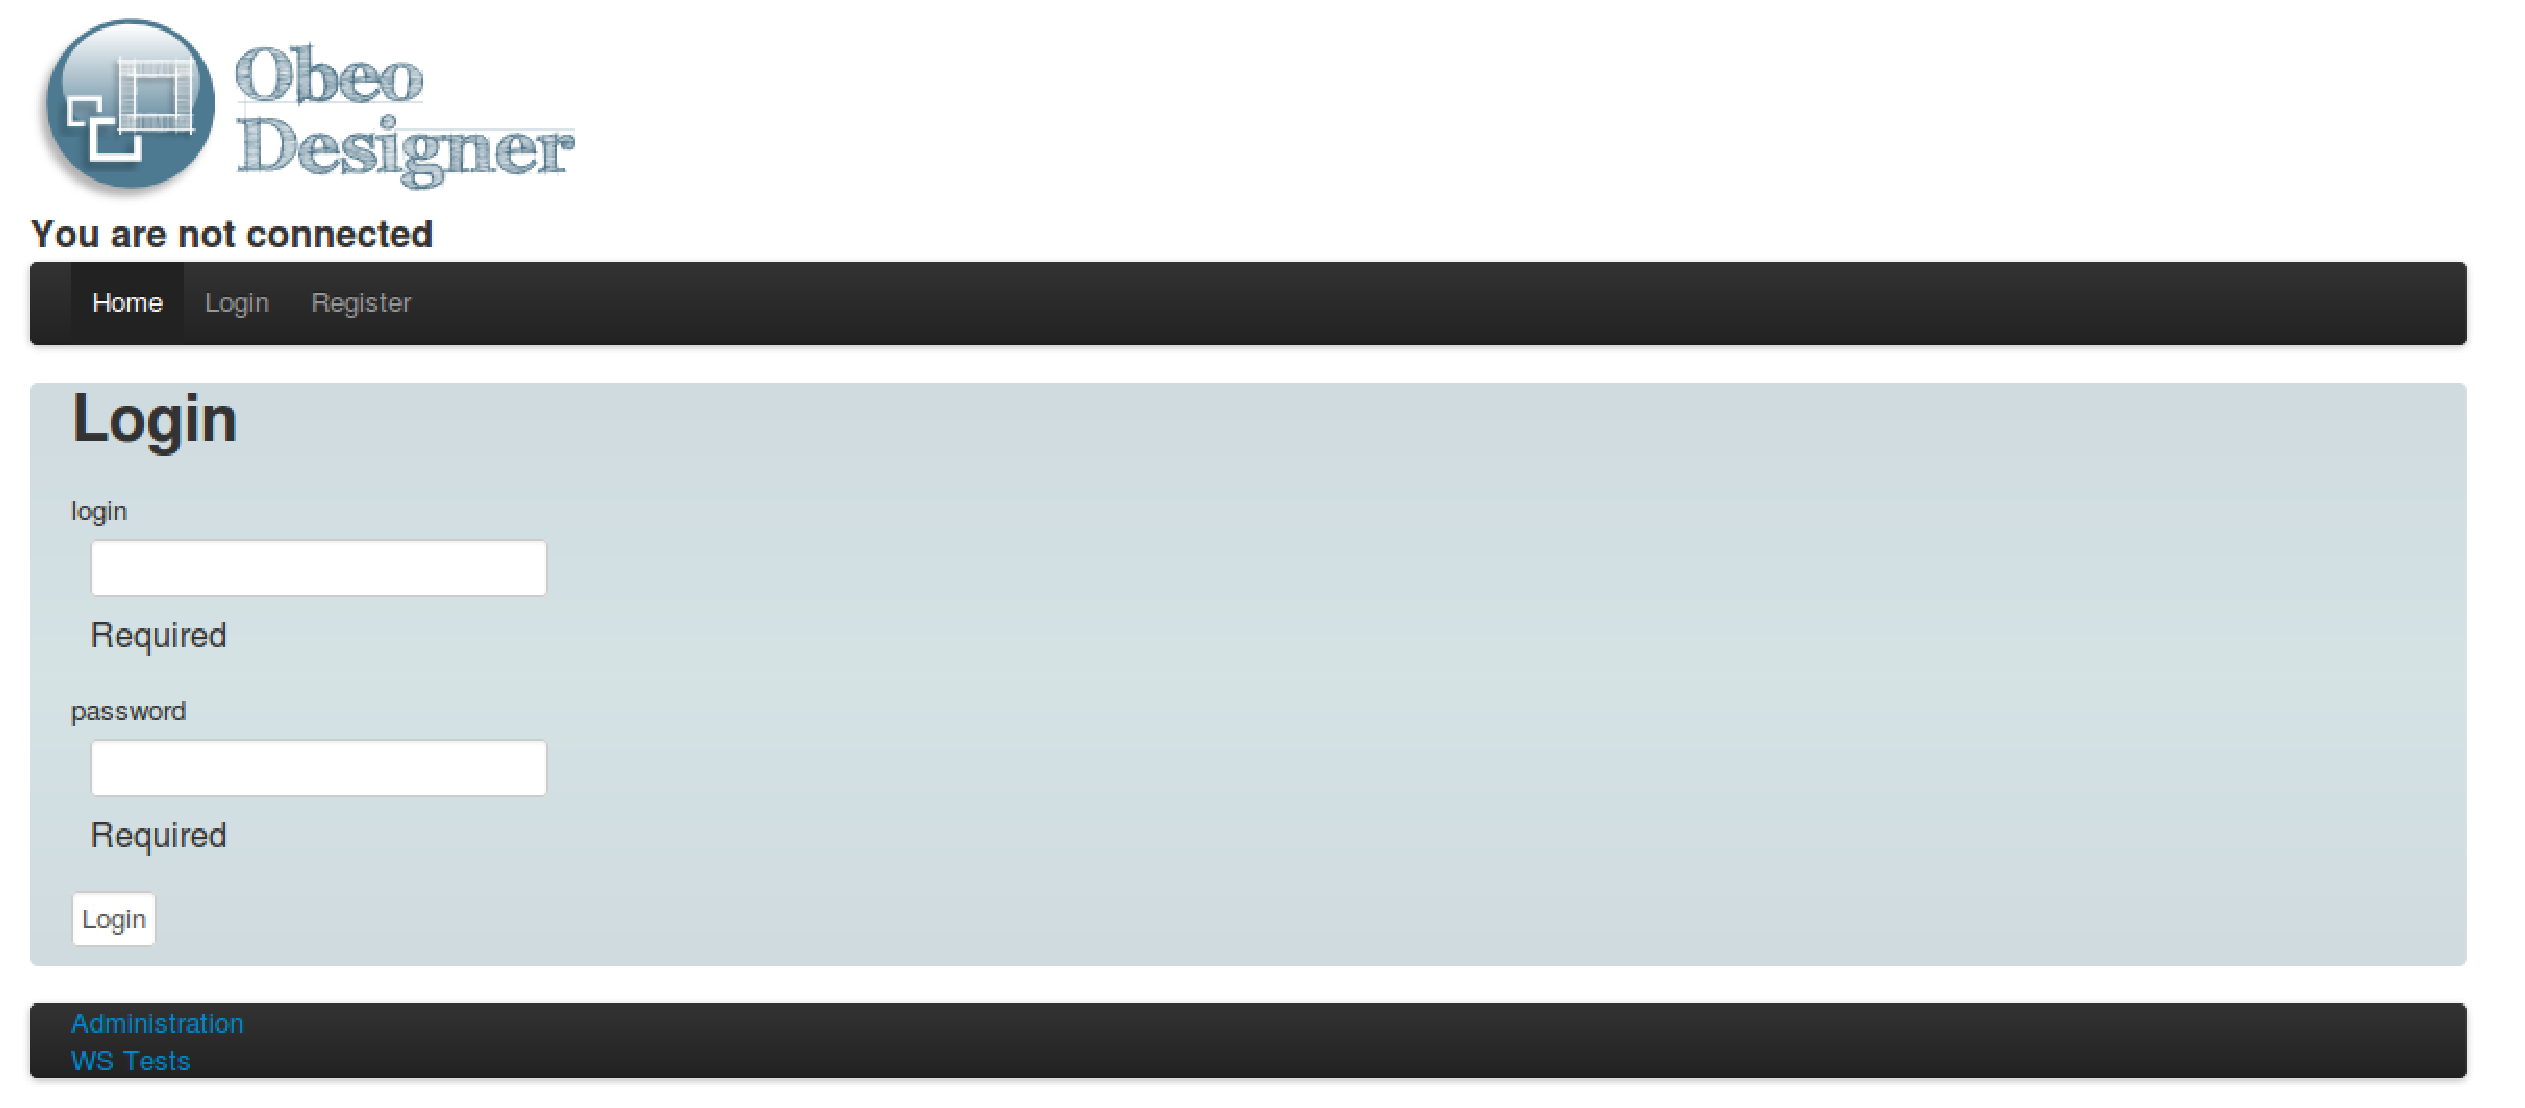
\includegraphics[scale=.4]{img/proto.eps}
  \label{Prototype Play_Shop }
  \label{fig:pro}
\end{figure}

